\documentclass[french]{article}
\usepackage[utf8]{inputenc}
\usepackage[T1]{fontenc}
\usepackage{babel}
\usepackage{biblatex}
\usepackage[draft]{graphicx}
\usepackage{csquotes}
\usepackage{parskip}
\usepackage{listings}
\usepackage[nopar]{lipsum}
\usepackage{hyperref}
\usepackage{fancyhdr}
\usepackage{xcolor}
\usepackage{enumitem} % for list
\usepackage[demo]{rotating} % rotating figure
\usepackage{glossaries}
\usepackage[toc,page]{appendix}

\makeglossaries

\newglossaryentry{siren}
{
    name=siren,
    description={Le siren (Système d'Identification du Répertoire des ENtreprises), est un code a 9 chiffres permettant d'identifier une entreprise ayant une activité sur le sol français.}
}

\newglossaryentry{nic}
{
    name=nic,
    description={Le nic (Numéro Interne de Classement) correspond aux 5 chiffres ajoutés au siren pour former le siret. Il permet d'identifier un établissement au sein d'une entreprise.}
}

\newglossaryentry{siret}
{
    name=siret,
    description={Le siret (Système d’Identification du Répertoire des ÉTablissements) est un code composé du siren et du nic permettant d'identifier les établissement de toutes les entreprises ayant une activité en France.}
}

\setcounter{secnumdepth}{6}

\pagestyle{fancy}
\setlength{\headheight}{13pt}

\definecolor{blue}{RGB}{51,131,255}

\addbibresource{bibliographie.bib}

\PassOptionsToPackage{hyphens}{url}\usepackage{hyperref}

\title{FRS Consulting - Rapport de stage}
\author{Pocquerusse Rémy - M1 MIAGE}
\date{Dates du stage : 03/04/2017 - 28/07/2017}

\begin{document}

\maketitle

\begin{center}
Encadré par Mr. Souheib Baarir et Mr. Gaétan Le Chat
\end{center}

\par\hfil\null\par
\par\hfil\null\par
\par\hfil\null\par
\par\hfil\null\par

\centerline{
\includegraphics[scale=0.7, draft=false]{frs_logo.jpg}}

\par\hfil\null\par
\par\hfil\null\par
\par\hfil\null\par

\begin{center}
{\huge Développement de User Stories sur}
\newline{}
{\huge \newline{une application Web}}
\end{center}

\clearpage

\renewcommand*\contentsname{Sommaire}

{\hypersetup{hidelinks}
    \tableofcontents
    
\clearpage

\section{Remerciements}

Je tiens à remercier tout particulièrement mon maître de stage, Mr. Gaétan Le chat, pour avoir partagé son expérience et ses conseils afin de me guider tout au long de mon stage.

Je remercie également l'équipe du projet, l'ambiance de travail et le partage de connaissances qui ont permis de créer un environnement optimal pour la réussite de mes missions.

Ces remerciements vont aussi à toute l'équipe de FRS Consulting pour leur accueil chaleureux et leur aide précieuse qui m'a permis de mieux comprendre le monde de l'innovation.

Enfin je remercie Mr. Souheib Baarir pour m'avoir encadré durant ce stage.

\clearpage

Note importante : le projet sur lequel j'ai travaillé est un projet actuellement en R\&D. Certaines informations confidentielles, mais néanmoins nécessaires à la compréhension, n'ont donc pas pu être intégrées à ce rapport. Il s'agit plus précisément de la définition du sujet, du but de mes missions, de données spécifiques de l'application et de son fonctionnement fondamental. Des annexes et des graphiques contenant des informations plus précises sur les parcours utilisateurs et la base de données ont également été enlevées.

\section{Introduction générale}

Selon le classement de Clarivate Analytics, la France se hisse en 2016 à la troisième place des pays les plus innovants, derrière les États-Unis et le Japon. Ainsi la France réaffirme sa position depuis de nombreuses années, et se définit comme un acteur majeur de l'innovation en Europe et dans le monde \cite{clarivate}. 
\newline{}
A cette dynamique s'ajoute une multiplication des incubateurs et accélérateurs qui ont permis, par exemple, à plus de 12 000 startups parisiennes de se développer en 2016 \cite{france-startup, france-startup2}.
\newline{}
La prise de conscience que l'innovation n'est, aujourd'hui, plus portée que par de grands groupes mais par une multitudes d'acteurs hétéroclites, a poussé l'Europe à encourager et favoriser les entreprises innovantes. De ce fait, la France et l'Europe ont multiplié les programmes d'aide à l'innovation, permettant à de plus en plus de projets novateurs d'être financés \cite{ent-gouv}.

Il existe aujourd'hui en France, plus de 200 dispositifs, français et européens, d'aide à l'innovation, accessibles à toutes les entreprises. Ce sont en effet plus de 80 Mds d'euro que l'Europe et la France consacrent à ces dispositifs. Seulement, ce foisonnement d'aides ressemble trop souvent à un maquis luxuriant, dans lequel seules les grandes entreprises, armées de financiers, arrivent à trouver leur chemin. En effet, plus de 80\% des aides sont drainées par ces grands groupes \cite{strategie-gouv-innov, eurostat}.

C'est dans ce contexte que FRS Consulting propose à ses clients d'étudier ces dispositifs à leur place. Elle met en relation ses clients avec des organismes financiers, proposant des dispositifs d'aide à l'innovation, et les accompagne dans leurs stratégies d'innovation.

\subsection{Choix du stage}

L'innovation est un secteur en mouvement, qui évolue constamment et qui se trouve par définition à la pointe de la technologie. C'est pour cela que c'est un secteur qui m'attire tout particulièrement.

J'ai eu plusieurs opportunités de stage. Tout d'abord Tkorp, une petite startup miagiste qui s'est lancée récemment dans la réalité virtuelle. Sa présentation, lors de son séminaire à l'Université Paris Nanterre, m'avait captivé. 
\newline{}
La réalité virtuelle est une technologie qui en est encore à ses balbutiements. Son utilité et ses possibilités dans divers domaines, tel que l'éducation sont encore à l'étude. C'est un secteur très dynamique et ouvert dans lequel travailler signifie souvent innover.
\newline{}
J'ai pu discuter d'un stage éventuel avec le président de Tkorp, Thibault Kerouanton, durant la nuit de l'info et lors d'un entretien téléphonique.
\newline{}
Malgré l'intérêt porté à ma candidature, le stage n'a finalement pas pu se faire, par manque de fonds et de priorités plus urgentes pour l'entreprise.

Avec le soutien de Mr. François Delbot, j'ai pu obtenir un entretien auprès de FRS consulting, une entreprise travaillant aussi dans le secteur de l'innovation.
\newline{}
FRS Consulting est un cabinet de conseil spécialisé en stratégie de l’innovation qui accompagne les entreprises innovantes dans la recherche de financement pour leurs projets. C'est également une Jeune Entreprise Innovante qui travaille actuellement sur une plateforme web, projet de R\&D stratégique de l'entreprise.

Mon choix de stage s'est porté sur FRS. En effet, le choix de cette entreprise comme organisme d'accueil s'est fait dans l'optique de découvrir un monde qui ne serait pas focalisé sur l'informatique, mais plus généralement sur l'innovation et la R\&D.
\newline{}
Le poste qui m'a été proposé se trouve dans le pôle R\&D de l'entreprise sous la tutelle de Gaétan Le Chat, directeur et chef de projet R\&D. Le sujet du stage se focalise sur la conception et le développement de nouvelles fonctionnalités pour la plateforme web.

\subsection{Thème et objectifs du stage}

Cette plateforme s'adresse à des entreprises souhaitant bénéficier d'une aide à l'innovation. Elle permet de fournir à FRS une visibilité et une attractivité accrues, et de favoriser le contact avec les clients.

Les fonctionnalités que j'ai eu à développer sur la plateforme concernent la partie récupération des données du client. Un utilisateur peut renseigner des informations et à partir de ces clés, nous pouvons récupérer les données de son entreprise via des API REST. La seconde partie correspond à l'analyse sémantique d'un texte pour en tirer des informations.
\newline{}
Le sujet du stage m'a tout de suite paru très intéressant car il ne se borne pas au développement d'une application, il intègre des phases de conception, tests, analyse du parcours utilisateur, recherche de solutions (notamment pour la seconde partie) et poussent à avoir une réflexion structurée et approfondie en amont et lors du développement.

J'ai donc choisi ce stage pour pouvoir mettre en pratique les nouvelles connaissances acquises lors de cette année de Master, les tester et les développer face à de nouvelles problématiques. De plus le stage me proposait de travailler sur de nouvelles technologies, en particulier sur des API REST et l'Open data qui sont je pense, une avancée majeure pour la recherche et l'évolution de notre société.

Ce rapport présente le stage que j'ai effectué au sein de l'entreprise FRS Consulting durant ces 3 derniers mois. Il a pour but de décrire le travail réalisé durant cette période, mais aussi d'analyser l'approche technique, humaine et organisationnelle que j'ai pu avoir lors de mes missions.

Depuis mon stage de L3, que ce soit à travers les cours ou les projets réalisés, j'ai acquis une vision de la conduite d'un projet informatique plus hétérogène, renforcée par les nouvelles technologies que j'ai pu appréhender.
\newline{}
C'est pourquoi le but de ce rapport n'est pas seulement de présenter les travaux réalisés, mais aussi de faire une analogie entre mon stage de Licence et de Master, afin de montrer l'évolution de ma démarche, lors de l'appréhension de problèmes inhérents à la conduite d'un projet informatique.

Nous présenterons tout d'abord l'entreprise, son marché, ses concurrents et sa vision de l'avenir.
\newline{}
Pour finir nous analyserons les technologies, le mode de gestion du projet, les missions effectuées lors du stage, les problèmes rencontrées, les solutions proposées et la démarche de développement.

\section{L'organisme d'accueil}

\subsection{FRS Consulting}

FRS Consulting, fondée en 2011, est un cabinet de conseil spécialisé en stratégie de l’innovation qui accompagne les entreprises, dans la construction d'une stratégie de croissance, leur permettant de financer leurs projets. FRS a été édifiée par des spécialistes du monde de l'innovation : Abdou Samb, Jean-Georges Fisher, Nicolas Raynaud, Cindy Meuric et Philippe Tonga. Issus de cabinets de conseil spécialisés dans le financement public de la R\&D et de l'innovation, leur conviction est que l'innovation est aujourd'hui un facteur clé pour la réussite et le rayonnement européen.
\newline{}
C'est de cette conviction que FRS Consulting est née, afin de contribuer à ce que l'Europe et ses entreprises s'assurent une compétitivité et une excellence scientifique qui sont les fondements de FRS.

L'entreprise est un des acteurs florissants dans le milieu français de l’innovation, et travaille en collaboration avec des organismes financeurs ou de contrôle tels que la Direction Générale des Finances publiques (DGFIP), le Ministère de l’enseignement Supérieur de la Recherche (MESR), la Banque Publique d’Investissements (BPI), la Compagnie Française d’Assurance pour le Commerce Extérieur (COFACE), la Caisse des Dépôts et Consignations (CDC), etc.

FRS s'implique encore plus fortement, dans l’écosystème français de l’innovation, en travaillant aussi aux côtés des pôles de compétitivité et des réseaux d’entrepreneurs, et contribue aux débats législatifs sur l’innovation en France et en Europe.

Le rôle de FRS est de pousser et de nourrir cette dynamique innovatrice française et européenne. Pour cela, elle assure aux entreprises un accompagnement dédié à des projets innovants afin de garantir leur succès.

De l'étude et la présentation d'un projet jusqu'à son financement, se déroulent plusieurs étapes qui font appel à des profils et des expertises différents. Ainsi, au sein de FRS, on distingue deux professions critiques : les consultants et les rédacteurs. Le rôle des consultants est d'accompagner les entreprises, tout au long des étapes nécessaires à l'obtention d'une aide. 
\newline{}
Les rédacteurs scientifiques possèdent une expertise dans le domaine principal du projet. Leur rôle est de rédiger la présentation du projet nécessaire à sa défense auprès des organismes financiers. Ainsi, ils doivent présenter et défendre, mais aussi analyser le projet pour assurer sa validation par les organismes financeurs.

\subsection{Les valeurs de l'entreprise}

Excellence, confiance et audace sont les 3 valeurs fondatrices de FRS Consulting.
\newline{}
Selon FRS, l'excellence passe par les méthodes de construction d'un projet innovant dans une PME. L'innovation doit se faire par étapes en établissant une stratégie solide de financement à moyen et long terme. Ce processus est unique pour chaque entreprise, car chaque projet est unique. Il s'applique à trouver les outils de financement adéquats, qui permettront à l'entreprise de baser son projet sur une réflexion durable et ainsi atteindre une excellence lui garantissant le succès. Le rôle de FRS est d'accompagner cette réflexion et de faire éclore des solutions pertinentes et novatrices.

Respect, confiance et transparence sont les codes que FRS établit avec ses clients et ses collaborateurs, car d'après FRS : ``l’Homme est la première richesse d’une organisation et la confiance, l’un des éléments fondamentaux de son adhésion à tout projet d’entreprise''.
La confiance reste la garantie d'une relation pérenne et profitable à tous.

L'audace, le talent et l'anticipation sont selon FRS indispensables à la réussite d'une entreprise dans le monde de l'innovation. FRS applique ces codes au sein même de son environnement.

\subsection{L'environnement FRS}

FRS évolue au sein d'un secteur très actif et changeant.
Afin de garder une dynamique au sein de son équipe, FRS fait participer les employés à des points flash permettant de discuter, de s'informer autour de l'actualité économique. Ils permettent aussi de palper l'ambiance au sein de l'entreprise, de discuter des difficultés, de l'organisation du travail, et du retour d'expérience avec les clients (questions compliquées auxquelles les consultants peuvent faire face). Les employés réfléchissent donc régulièrement aux meilleures approches à adopter pour proposer de nouvelles idées à leurs clients.
\newline{}
L'autre point fort est la logique d'anticipation du marché qui prend une place prépondérante dans les discussions, afin de rester précurseur en matière de consulting.

\subsection{Contexte concurrentiel}

Selon l'ACI (Association des Conseils en Innovation), on dénombre aujourd'hui environ 70 entreprises qui sont spécialisées dans l'accompagnement de l'innovation \cite{aci}. Cette profession est relativement nouvelle, beaucoup de ces entreprises sont jeunes même si certains grands groupes possèdent leur propre pôle d'accompagnement. C'est un secteur en pleine croissance, attractif, porté par une population jeune et dynamique.
\newline{}
FRS reste donc en concurrence avec bon nombre de ces entreprises, notamment des grands groupes comme Ayming, Leyton ou F.Iniciativas. Ces grands groupes sont importants en France mais aussi en Europe et dans le reste du monde. Ce ne sont pas des entreprises spécialisées dans l'accompagnement de l'innovation, mais elles disposent chacune de ressources et d'une expertise conséquentes.

Le marché permet néanmoins à des entreprises nouvelles d'émerger et de concurrencer ces grands groupes, ce sont des entreprises comme FRS Consulting ou encore Monte Cristo Consulting. Ces entreprises doivent cependant se différencier et innover continuellement, pour pouvoir grandir et évoluer, dans un marché en plein essor qui voit de nouveaux acteurs arriver chaque année.

\subsection{La plateforme web}

Cette plateforme doit répondre au problème qui se pose sur le nombre et la complexité des dispositifs d'aide à l'innovation. Un utilisateur n'aura pas forcément la patience ou les connaissances pour évaluer chaque dispositif en fonction des besoins de son projet.
\newline{}
Mon travail s'inscrit pleinement dans le cadre du développement de la plateforme car nous avons besoin de connaître et comprendre les besoins de l'entreprise.

Cette plateforme doit être, à l'avenir, un carrefour pour tous les acteurs de l'innovation et permettre à FRS de se distinguer de la concurrence. Ce projet représente donc un avantage stratégique important. En effet la plateforme est, pour FRS Consulting, un atout majeur face à la concurrence.

\section{Technologies}

\subsection{Django}

\subsubsection{Le framework Django}

Django \cite{django} est un framework Pyhton axé web qui apporte une toute nouvelle vision de la gestion du développement d'un site web. Il encourage les développeurs à travailler rapidement et efficacement afin de concrétiser un projet le plus vite possible. Pour ceci, il prône le principe DRY (Don't Repeat Yourself) qu'il applique à travers sa structure et sa philosophie de développement. Mais sa plus grande force réside dans l'automatisation et la gestion d'un grand nombre de tâches et fonctionnalités. Certaines de ces fonctionnalités ont su rendre ce framework populaire auprès d'un grand nombre de développeurs. Plus précisément, les principales fonctionnalités de Django sont les suivantes :

\begin{enumerate}
    \item La génération d'une interface via son api d'abstraction des données permettant une administration des données simplifiée. La gestion de la base de données peut se faire via une interface générée automatiquement et entièrement paramétrable.
    \item La création de la base de données se fait entièrement en Python à travers les modèles et les méthodes apportées par Django. Il en résulte une création de la base facilitée et beaucoup plus dynamique. Les interactions avec la base se font via des méthodes dédiées.
    \item Une gestion des urls sous la forme d'un index qui permet de mapper simplement une url avec une vue (une page dynamique).
    \item Sécuriser son application contre les injection SQL, le Cross-Site Request Forgery ou encore le clickjacking se fait facilement avec Django, ce qui permet d'éviter des erreurs assez communes.
    \item La capacité à gérer une affluence très importante n'est plus à prouver, des sites comme Youtube, Reddit et même Google utilisent cette technologie.
\end{enumerate}
Ce sont toutes ces fonctionnalités, et bien d'autres, qui ont contribué au succès de Django.

\subsection{L'Open Data et les Api REST}

En 2013, lors du sommet du G8, la « Charte du G8 pour l'ouverture des données publiques »  a été ratifiée. Ainsi les collectivités se voient dans l'obligation de publier des données publique au format numérique. \cite{wiki-open-data}

Ceci a permis en outre l'ouverture de données publiques sur les entreprises, la recherche, etc... Mais a aussi permis d'encourager différents services à accélérer l'ouverture de leurs données.
Certaines de ces collectivités fournissent des services entièrement dédiés en mettant en place des api REST.

Une api REST ou RESTful (REpresentational State Transfer) est un style d'architecture pour les systèmes hypermédia permettant de construire des application tel que le web, un intranet etc... De plus en plus de services proposent des apis avec lesquelles on peut interagir. C'est un concept créé en 2000 par Roy Fielding dans le chapitre 5 de sa thèse de doctorat. \cite{roy}
\newline{}
Une api REST permet une interaction avec un utilisateur via des requêtes HTTP permettant de travailler sur les données stockées en utilisant des requêtes comme GET ou POST.
\newline{}
Travailler avec une api REST se fait via un ensemble de fonctions sur lesquelles un développeur peut effectuer des requêtes et recevoir une réponse contenant les données sous un format prédéfini (le plus souvent Json).

Pour illustrer le fonctionnement d'une api REST prenons par exemple Datainfogreffe. Je souhaite obtenir des informations de l'entreprise dont le siren est : 383474814 (il s'agit de Airbus) et récupérer ses données financières en 2015. Pour cela je construis une requête satisfaisant mes critères :
\url{https://datainfogreffe.fr/api/records/1.0/search/?dataset=chiffres-cles-2015&q=siren%3D383474814}
\newline{}
Les données récupérées peuvent ensuite être traitées.

Ayant travaillé ou exploré plusieurs apis REST, notamment Datainfogreffe et scanR, j'ai pu me faire une idée sur les forces et les faiblesses d'une api. Le travail effectué sur Datainfogreffe puis sur scanR, qui sont des plateformes ayant chacune leurs points forts et leurs points faibles, m'a clairement montré les bonnes pratiques à suivre. 

Le point faible de Datainfogreffe réside dans sa structure qui ressemble trop à la vision que pourrait avoir un comptable d'une organisation cohérente des données. L'api se divise par année et par thème. A chaque année correspond un certain nombre de jeux de données (informations financières, immatriculations, etc...). Cette structure ne pose aucun problème si l'on sait à l'avance ce que l'on recherche. Dans le cas contraire, la recherche d'information se transforme en une suite de nombreuses requêtes. En effet il faut chaque année rechercher dans chaque jeu de données pour obtenir une information. De plus, la structure de ces jeux de données diffère en fonction de l'année et du jeu de données. Ce qui implique de connaître la structure de chaque jeu de données de chaque année.

Contrairement à Datainfogreffe, c'est dans sa structure que scanR trouve son point fort. ScanR ne possède qu'un jeu de donnée permettant de rechercher des informations. Une recherche efficace est donc faisable avec une simple requête.

Néanmoins, la documentation de Datainfogreffe reste très fournie. Elle est claire, détaillée et permet de prendre en main l'api très facilement. De plus, Datainfogreffe dispose d'une véritable interface permettant la construction de requêtes, ce qui facilite grandement la prise en main de l'api.
\newline{}
C'est ce qui fait grandement défaut à scanR qui ne dispose d'aucune documentation. Son swagger (interface permettant de manipuler l'api) fait office de documentation et d'interface permettant le dialogue avec l'api. La prise en main reste donc compliquée même si à terme sa manipulation est très ergonomique.

De cette expérience j'ai pu établir plusieurs points vitaux permettant de développer efficacement une api REST. 

Tout d'abord sa structure se doit d'être simple, ne pas subdiviser l'api en différents jeux de données qui, pourtant, possèdent des informations liées.
La solution à ce problème qui est à la fois plus adaptée et plus maintenable est de structurer efficacement les données retournées.
Par exemple avec Datainfogreffe, plutôt que de diviser les datasets de l'api par année, il suffit de diviser les données retournées par année. Le développeur n'effectue plus qu'une seule requête et peut parcourir à sa guise les données de chaque année. Cela permet aussi de garder une structure des données plus uniforme et cohérente avec le reste des jeux de données.

L'api doit être developer-friendly, c'est-à-dire explorable via le navigateur et/ou proposer une interface pour la construction de requêtes. Cela permet de prendre en main rapidement et efficacement les fondamentaux de l'api et de faciliter les phases de test.

La documentation reste indispensable pour tout type de projet. Sans documentation, une api n'invite pas le développeur à l'explorer. Dans ma première mission, l'utilisation de scanR a été reportée à cause du manque de documentation. Un swagger peut remplacer une documentation s'il est bien construit et assez fourni, pour donner à l'utilisateur tous les éléments nécessaires à une utilisation efficace de l'api.

\section{Travaux effectués}

\subsection{Mise en place et gestion du projet}

Jusqu'à mon arrivée, le projet n'était développé que par mon tuteur. Le travail se faisait donc directement en local, sans gestion de versions. La mise en place d'un gestionnaire de versions m'a tout de suite semblé indispensable, avant de commencer à travailler sur le projet. Ce gestionnaire devait proposer d'héberger un projet privé, gratuitement. La plupart des gestionnaires de versions sont payants lorsqu'il s'agit d'héberger un projet privé. J'ai pu trouver plusieurs solutions, dont Gitlab. \cite{gitlab} En plus de satisfaire les conditions requises, il intègre une fonction permettant l'intégration continue, un gestionnaire de bugs performant et une documentation intégrée au projet qui sont des plus face aux concurrents comme bitbucket.
\newline{}
D'autre part, j'ai pu proposer différents logiciels de suivi et de gestion de projets permettant de faire de l'intégration continue (GitLab, Jenkins), le suivi de la qualité de code et de la couverture des tests (Codecov, Codacy, sonarQube, Coveralls) et d'un suivi des tâches (Jira, Trello). Cependant, mon tuteur n'a pas jugé nécessaire de mettre en place trop d'outils pour la gestion du projet, préférant la communication orale et éviter d'ouvrir le projet à trop d'applications externes. 
\newline{}
En outre, jusqu'ici, le développement se faisait sous vim. Avec l'adoption d'un gestionnaire de versions et python étant très sensible à l'indentation, il m'a semblé indispensable d'intégrer un IDE dans le processus de développement. Un IDE permet une gestion des versions beaucoup plus simple (en particulier en cas de conflit) et une accélération du processus de développement. La gamme de Jetbrains proposant un éditeur pour python (PyCharm) supportant Gitlab, il a tout de suite été adopté.

Les développeurs se trouvant dans le même bureau, la communication autour du projet était assez active. Le suivi du projet se faisait selon la méthode Scrum, avec une réunion chaque semaine, afin d'évaluer l'état d'avancement du projet. Lors de ces réunions, chaque développeur présente le travail effectué durant les derniers jours et discute des points d'amélioration, des éventuels problèmes liés à la conception ou au développement de l'application. Ensuite, le travail à effectuer pour la semaine est établi. Lorsqu'un développeur estime avoir achevé une partie plus ou moins importante de l'application, il peut la présenter aux autres développeurs pour opposer différents points de vue sur l'esthétique, le parcours utilisateur, et la conception de l'application.

\subsubsection{L'équipe}

L'équipe travaillant sur la plateforme est très hétéroclite car ses besoins sont très techniques et nécessitent une analyse poussée du marché. Ainsi il y a 6 personnes travaillant actuellement sur la plateforme :

\begin{itemize}
    \item Gaétan Le Chat : chef de projet R\&D, il est en charge de la gestion et du suivi du projet, des spécifications techniques et fonctionnelles et du développement.
    \item Kymble Christophe : doctorant en économie, il s'occupe de la recherche de solutions et l'évaluation des différents dispositifs nécessaires au projet
    \item Huu-Hiep Huyn : développeur frontend, il gère la restructuration du projet, refonte du design, mise en forme des données, etc...
    \item Alice Moisson : elle est le soutien technique de Kymble
    \item Amokrane Zatout : il est le soutien technique de Kymble
\end{itemize}

\subsubsection{Gitlab}

Avec Gitlab, il a fallu choisir un workflow approprié au développement du projet. Gitflow m'a paru être une méthode adaptée sur laquelle s'appuyer. C'est un workflow très complet qui permet de gérer la majorité des cas rencontrés lors du développement. C'est surtout un workflow simple à comprendre, permettant une gestion du projet en profondeur. \cite{workflow}

Basé sur gitflow, notre workflow se découpe en plusieurs branches. La branche master qui contient l'application sous sa version stable et accessible aux utilisateurs. Une branche développement contenant les nouvelles fonctionnalités de l'application à intégrer et tester. Elle sert aussi de branche de déploiement des nouvelles fonctionnalités. Enfin, des branches de fonctionnalité, généralement une par développeur, pour chaque nouvelle fonctionnalité à réaliser.

Ce mode de fonctionnement simplifie grandement le travail du développeur car il ne travaille qu'avec sa propre branche et la branche de développement.

\subsection{Mission 1 - Récupération de données}

Le but de cette mission est de récupérer les données critiques d'une entreprise en utilisant différentes api REST. Ces données sont ensuite revues par l'utilisateur. 

Deux actions sont a effectuer :

\begin{enumerate}
\item Garantir la véracité des données et leur prescription. 
\item Gérer l'organisation des données. Le nombre de données à collecter est relativement conséquent. Un utilisateur n'aura ni la patience ni l'envie de rechercher et de renseigner toutes ces données.  
\end{enumerate}

\subsubsection{Conception de l'application}

\paragraph{Les apis REST}
La base de données devait être conçue de manière à contenir, en grande partie, des informations issues des api, notamment Datainfogreffe, afin d'éviter tout problème d'intégrité des données.

\enquote{Datainfogreffe a été créé par le G.I.E. Infogreffe pour permettre aux greffiers des Tribunaux de commerce, officiers publics et ministériels, d'assurer une plus large diffusion de l'information légale sur les entreprises. Le portail Datainfogreffe a pour objectif d'augmenter le potentiel de création économique des entreprises, en mettant à leur disposition des données dans des formats ouverts et facilement réutilisables.} \textit{\url{https://data.infogreffe.fr/page/faq/}}

Datainfogreffe permet ainsi de consulter les données d'entreprise qui ont été ratifiées par un greffier garantissant leur validité. L'api s'organise de manière annuelle, à chaque année correspond un certain nombre de datasets (jeu de données). Ces datasets sont organisés en fonction des entreprises radiées, immatriculées ou des chiffres clés (informations financières) etc, ... 
\newline{}
Les datasets à utiliser sont ceux permettant d'obtenir les informations nécessaires à la construction du profil de l'entreprise. Les informations contenues dans les datasets des entreprises immatriculées et des chiffres clés sont à la fois les plus complètes et les plus fournies.

Une seconde version de Datainfogreffe est en développement, elle est actuellement dans sa version bêta. Il a été décidé de ne pas en tenir compte durant le développement mais de faire néanmoins une veille afin d'anticiper une refonte de l'application vers la nouvelle api. Le développement s'est fait sur la première version de l'api afin de garantir des outils exempts de bugs.

Durant le développement, il a été décidé d'utiliser une seconde api REST cette fois-ci basée sur la recherche et l'innovation. L'api scanR regroupe en effet différentes informations liées à l'innovation, que ce soit autour des entreprises, d'associations ou des laboratoires de recherche. On peut y trouver les différents brevets déposés, les publications ou encore les projets R\&D. \cite{scanr}

\paragraph{Cas d'utilisation - Utilisateur}

Les cas d'utilisation ci-dessous sont ceux qui m'ont été demandés et m'ont servi de référence pour la conception de l'application. Nous verrons ensuite les problèmes rencontrés, liés à ces cas d'usage.

Du point de vue d'un utilisateur, l'application se doit d'être simple. Il peut emprunter différents chemins lors de l'exploitation de l'application. Il peut soit utiliser la recherche d'entreprise, soit remplir le formulaire manuellement.

S'il décide de remplir les données du formulaire sans utiliser l'auto-complétion, ou si aucune donnée n'a été trouvée sur son entreprise, il faut pouvoir lui afficher le formulaire. En effet, afin d'encourager les utilisateurs à recourir à la recherche d'entreprise, et d'obtenir un maximum d'informations, le formulaire reste tout d'abord caché. L'utilisateur peut décider ou non d'afficher le formulaire. Une fois le formulaire affiché, il doit le remplir avant de valider et de passer à la description du projet. Le cas où l'utilisateur décide de faire une recherche est défini ci-dessous :

L'utilisateur doit pouvoir rechercher une entreprise, choisir son entreprise parmi les résultats affichés, vérifier et corriger le formulaire pré-rempli. 

\paragraph{Cas d'utilisation - Application}

L'utilisateur peut décider de remplir le formulaire manuellement. Dans ce cas, le travail du serveur est seulement de valider et d'enregistrer les formulaires. En revanche, dans le cas où l'utilisateur décide de rechercher une entreprise, les interactions entre les apis et la construction du formulaire sont plus complexes. 

En effet si un utilisateur effectue une recherche, le serveur doit aller récupérer les données les plus récentes dans la base de données ou Datainfogreffe, et les afficher à l'utilisateur. L'application doit rechercher les données dans la base puis sur Datainfogreffe. S'il n'y a aucune information sur l'entreprise dans la base, on regarde dans tous les datasets de Datainfogreffe. S'il y a une entrée dans la base, on va alors chercher dans les datasets postérieurs à la date de l'entrée. On affiche ensuite les données les plus récentes, et on enregistre le formulaire après validation par l'utilisateur.

\subsubsection{Une conception à revoir}

Très vite, avant et durant le développement, je me suis aperçu que certaines demandes étaient mal conçues. Ainsi, lorsqu'un utilisateur souhaitait rechercher une nouvelle entreprise, l'application devait faire une comparaison entre les données présentes dans la base, et celles présentes dans Datainfogreffe, afin d'afficher à l'utilisateur les données les plus récentes. Si 2 utilisateurs décident, que ce soit l'un pour tester l'application, et l'autre pour réaliser une recherche plus sérieuse sur la même entreprise. Les données de la base se verraient partagées entre les 2 utilisateurs, ce qui peut amener une incompréhension pour l'utilisateur et des données altérées pour la base. Le but est de toujours afficher à l'utilisateur les données les plus récentes possibles. Les données de la base doivent en revanche rester en interne et ne pas être partagées à tous les utilisateurs.

\begin{figure}[ht]
\centering
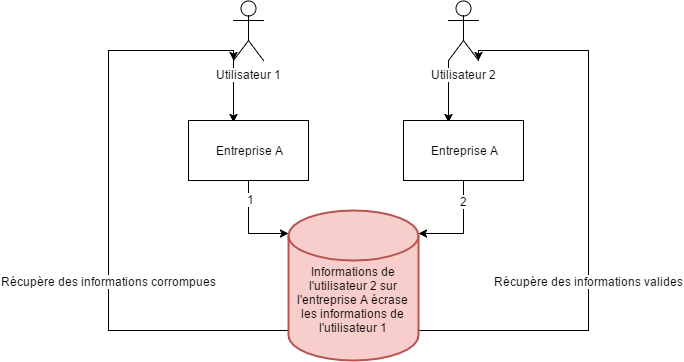
\includegraphics[width=\textwidth, draft=false]{data_problem.png}
\caption{Les données des entreprises peuvent être altérées}
\label{fig1}
\end{figure}

Pour palier à ce problème, j'ai proposé la mise en place de cookies. Lorsqu'un utilisateur se connecte afin de faire une nouvelle recherche ou consulter une recherche précédente, le formulaire est déjà pré-rempli avec les données de sa recherche précédente. Ce qui permet de pallier au problème de la fraîcheur des données. En effet, les données affichées à l'utilisateur sont toujours celles qu'il a manipulées.

Ainsi, lorsque 2 utilisateurs travaillent sur la même entreprise, ils n'ont en commun que les données enregistrées dans la base. Ces données peuvent donc être altérées mais seulement en partie (l'utilisateur ne peut modifier que les données principales de l'entreprise, son adresse, et ses données financières les plus récentes). Cela peut se résoudre de diverses manières comme identifier une entreprise de façon plus précise. Mais il a été décidé d'utiliser l'historisation des données fournies par Django.

De plus, certaines entreprises préfèrent payer une amende plutôt que de divulguer leurs informations (financières notamment). Ainsi se pose la question de l'anonymat d'un utilisateur. Sachant que l'utilisateur n'a pas besoin de se logger, comment identifier un utilisateur et par extension une entreprise effectuant une recherche sur la plateforme ? Ici on considère l'utilisateur anonyme lorsqu'il n'entre pas d'informations permettant d'identifier son entreprise (nom/nic ou siren). L'identification d'un utilisateur, ne serait-ce que pour pouvoir suivre sa démarche ou à des fins statistiques, est importante. Cependant sans authentification le suivi des utilisateurs est compliqué. A ce jour, aucune méthode précise n'existe pour identifier de manière sûre un utilisateur, surtout sur un parcours aussi court que l'enregistrement de données. Il a donc été décidé d'utiliser plusieurs clés d'identification. Tout d'abord le nom de l'entreprise qui est obligatoire ; en effet, un utilisateur aura tendance a utiliser le même nom pour ses différentes recherches. Ensuite l'adresse IP de l'utilisateur qui permet d'ajouter un nouveau filtre pour une identification plus précise. L'adresse retournée sera souvent une adresse publique, mais certaines adresses permettent d'identifier de façon plus ou moins précise la localisation de l'utilisateur. Enfin, pour situer une recherche dans le temps, un timestamp a été ajouté permettant aussi de différencier les multiples entrées d'un utilisateur.
Ainsi une entrée est de la forme : nom:127.0.0.1:1498045519.

Tout ceci, et la prise en compte de l'api scanR, a entraîné une modification du cas d'utilisation de l'application.

\paragraph{Cas utilisation 2 - Application}

Ainsi le cas d'utilisation a été modifié de la façon suivante :

Si un utilisateur effectue une recherche, le serveur doit aller récupérer les données correspondantes sur Datainfogreffe et les afficher à l'utilisateur. Si aucune entreprise ne correspond, on effectue  alors une recherche sur scanR. Si aucune donnée n'est présente, on propose à l'utilisateur de remplir le formulaire manuellement. 

Dans le cas où les données sont présentes sur Datainfogreffe, on va tenter de les compléter avec scanR (notamment pour l'adresse et la géolocalisation qui sont plus précises sur scanR que sur Datainfogreffe), puis on affiche le formulaire pré-rempli. Dans le cas où les données sont seulement présentes sur scanR, on affiche le formulaire pré-rempli. Lors de l'enregistrement des formulaires, s'ils ont été remplis manuellement ou par l'intermédiaire de Datainfogreffe, on enregistre dans la base. Si scanR a été utilisé pour générer le formulaire, alors on récupère les données complémentaires de l'entreprise.

\paragraph{Base de données}

Il faut penser la base en reprenant la structure d'une entreprise et les données disponibles sur Datainfogreffe et scanR. Chaque entrée possède un identifiant (id) géré automatiquement par Django. Les règles de relation entre les tables ont été mises en place afin de prendre en compte la complexité des entreprises.

\paragraph{Avant de développer, penser à l'évolution de l'application} Cette application est appelée à évoluer, de nombreuses api seraient en mesure de l'enrichir mais ne sont actuellement qu'en phase de développement ou en phase de test. Il faut donc tout d'abord penser l'application en facilitant l'intégration de nouvelles api. Il faut aussi prévoir l'évolution de ces api, par exemple, chaque année, Datainfogreffe revoit les intitulés de ses données. Le but est donc de réaliser une application à la fois maintenable et évolutive. 

Il existe une infinité de méthodes et de procédés permettant d'accomplir une mission. Ces méthodes sont bonnes ou mauvaises. Le plus important avant et lors du développement, est de définir et faire évoluer la meilleure méthode permettant d'accomplir la mission. Ce comportement est essentiel pour conduire une mission à terme, en fournissant une application maintenable, évolutive et intelligente.
\subsubsection{Développement}

\paragraph{Travailler avec Datainfogreffe}

Lors du développement j'ai voulu me familiariser avec l'utilisation d'une api REST, afin de mieux appréhender le développement de l'application et les différentes possibilités de conception. J'ai donc établi une feuille de route pour la récupération d'une donnée spécifique. Sachant que j'ai un siren, permettant d'identifier de façon unique une entreprise sur Datainfogreffe, comment récupérer ses données les plus récentes et comment les organiser ?
\newline{}
Le problème de Datainfogreffe se présente dans sa structure et dans le nombre de requêtes à effectuer afin d'obtenir ces informations. Comme décrit plus haut, le fonctionnement de Datainfogreffe se fait par année. Chaque année, il y a au plus 2 datasets susceptibles de nous intéresser. Datainfogreffe couvrant les données des entreprises de 2012 à 2017, il y a donc potentiellement 10 requêtes à effectuer pour obtenir les informations d'une seule entreprise ou d'un groupe d'entreprises.

\begin{figure}[ht]
\centering
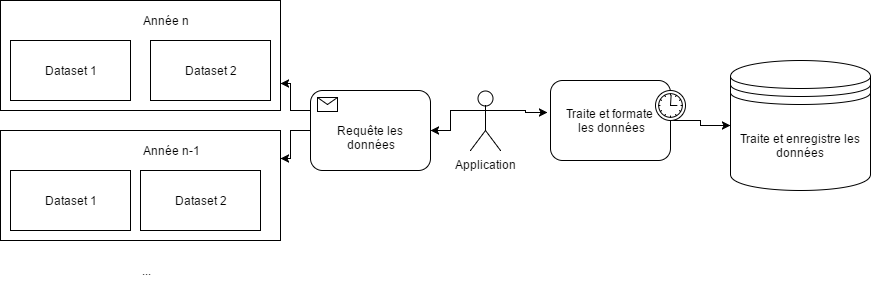
\includegraphics[width=\textwidth, draft=false]{api_diagram.png}
\caption{Process de récupération des données}
\label{fig2}
\end{figure}

Seulement, entre chaque année et chaque dataset, les données définies ne se recoupent pas forcément, et la syntaxe utilisée pour décrire ces données diffère plus ou moins. Or cette syntaxe est vitale pour manipuler les données. Il faut donc pour chaque set de donnée, créer un test conditionnel sur leur syntaxe afin de s'assurer de toujours manipuler des données cohérentes et complètes (voir annexe : \ref{appendix:infogreffe_json_compare}).

Pour ce faire, j'ai décidé de créer un jeu de ressources contenant les intitulés de chaque donnée importante. Datainfogreffe changeant ses données chaque année, j'ai tout d'abord pensé à le générer automatiquement. Il n'existe cependant aucune manière à travers l'api de récupérer ces informations concernant les datasets. J'ai donc dû établir moi-même les dénominations de chaque donnée. Ce fichier de ressource se présente ainsi : pour chaque groupe de donnée, on crée un dictionnaire contenant les intitulés.
\newline{}
Cette méthode permet plusieurs choses, tout d'abord elle évite de faire une suite de tests conditionnels très redondants. Ensuite, elle est facilement maintenable car si les intitulés des données changent de nouveau, il suffit simplement de les rajouter en créant de nouvelles entrées dans les dictionnaires.


\paragraph{Construire la base}

La création de la base de données et de son modèle logique se fait dans la classe Models de Django. Un modèle, ou une table, définit une source d'information durable à propos de donnée. Un modèle est une classe Python où chaque attribut représente un champ de la base. Le modèle logique et la structure de la base sont donc entièrement définis dans l'application.

La structure de la base se définit simplement car les tables de relation sont gérées par Django. Prenons l'exemple du modèle d'une entreprise et des brevets. Une entreprise peut avoir plusieurs brevets et un brevet peut être possédé par plusieurs entreprises. On a donc une relation plusieurs à plusieurs. Pour que cette relation soit prise en compte dans la base, il suffit de déclarer un champ ManyToMany dans l'un ou l'autre des modèles. 

Il est possible de définir tous les éléments nécessaires à une gestion de la base en profondeur, en particulier pour la validation des données. En effet, nombre de champs sont définis par des codes de l'INSEE et possèdent donc des règles d'écriture strictes, comme le \Gls{siren}. Ainsi Django intègre des validateurs (expressions logiques) directement dans les modèles, cela permet d'apporter une sur-couche dans la validation des données.

Comme précisé précédemment, la base est destinée a être peuplée en partie par les données des apis et par les utilisateurs. Or, les données reçues sont potentiellement instables. Il a donc fallu en tenir compte dans la création de la base. Ainsi très peu de champ sont obligatoires et une entreprise peut, potentiellement, n'avoir aucune relation avec les autres modèles.

\paragraph{Une application dynamique}
L'application se voulait être à la fois simple d'utilisation et dynamique afin d'amener l'utilisateur à son but le plus rapidement possible. Ainsi lorsque l'utilisateur performe des actions : recherche et sélection d'entreprise, l'application ne redirige pas l'utilisateur vers une succession de pages qui pourrait donner l'impression d'une suite d'étapes fastidieuses.

Cette dynamique est gérée par Ajax. Cela permet d'éviter la transmission d'une page HTML complète et de n'en rafraîchir qu'une partie. Le problème avec cette conception est le transport des données entre le serveur et le client. 

L'application se construit autour de 3 templates. Un template principal qui définit la structure de l'application, un template secondaire qui étend le template principal et gère l'affichage du formulaire. Enfin un template inclus dans le template secondaire qui permet de gérer les formulaires et leurs contenus. Cette structure permet de ne jamais régénérer entièrement une page.

Lorsque l'utilisateur recherche une entreprise, le serveur renvoie les résultats. Cette requête est traitée simplement, comme un formulaire. Ici l'utilisation d'Ajax n'a pas semblé nécessaire, car l'utilisateur est redirigé instantanément vers la même page, et les données permettant le choix de son entreprise s'affichent directement. L'utilisateur n'a donc à aucun moment l'impression d'avoir quitté la page.

Lors du choix de son entreprise, on ne peut traiter la requête de l'utilisateur sans le rediriger vers une nouvelle page. Ainsi, pour envoyer la requête et gérer les données reçues, on utilise Ajax. Lorsque l'utilisateur sélectionne son entreprise, on envoie une requête Ajax contenant les données des entreprises et le siren de l'entreprise sélectionné. On affine ensuite les données en fonction du siren et on pré-remplit les formulaires qui sont renvoyés. De cette manière, seule la partie formulaire de l'application est rechargée.

Ceci est possible en se basant sur une autre fonctionnalité de Django, les templates. Un template ou gabarit est un système agile de génération dynamique de code HTML. Un template est représenté par une partie HTML statique qui construit la structure fondamentale d'une page. Et par une partie dynamique. Cette partie dynamique permet, via une syntaxe particulière, d'ordonner et afficher les données reçues.

\paragraph{Construire les bases de l'application}

Ce style d'application nécessite d'utiliser une seule vue (hub permettant de gérer les requêtes de l'utilisateur et de lui retourner les templates correspondants) gérant les différentes requêtes de l'utilisateur. Une vue est une fonction Python acceptant pour paramètre une requête Web et qui renvoie une réponse Web. Cette réponse peut être du code HTML, une redirection, etc...

Dans Django, une vue correspond à une URL, il est donc impossible de gérer les différentes requêtes avec différentes vues. Ainsi la vue doit pouvoir identifier les requêtes et gérer les données des templates à renvoyer à l'utilisateur.

L'identification d'une requête se fait en fonction de son type et de son contenu. Il est possible de différencier une requête POST d'une requête Ajax mais aussi de différencier les différentes requêtes POST ou Ajax en y ajoutant des informations complémentaires (identifiants des formulaires par exemple).

La vue dispose donc de différents chemins possibles dont chacun détermine un parcours utilisateur. Les données retournées et les traitements effectués sur les requêtes de l'utilisateur sont déterminés par ces parcours. 

Lors de sa première connexion, l'utilisateur est redirigé vers le template principal, permettant d'afficher une page avec le formulaire de recherche et les formulaires cachés permettant d'entrer les informations de l'entreprise.

L'utilisateur peut effectuer différentes actions, connexion à la page, recherche d'entreprise, sélection d'entreprise et édition d'un formulaire contenant les informations de son entreprise.

\paragraph{La recherche d'entreprise}

Dans Django, la création et la gestion des formulaires se fait côté Backend. La classe Form de Django décrit la structure d'un formulaire, son fonctionnement et son apparence. Ce formulaire est ensuite incorporé dans la création du template. 

Pour la recherche d'entreprise, il suffit d'un simple formulaire avec un seul input. Ce formulaire est censé recevoir des données complètement différentes, on ne peut donc faire aucune validation pour s'assurer que les données récupérées côté client soit correctes.

La recherche dans les datasets de Datainfogreffe se fait par ordre décroissant, de l'année courante à 2012. On va commencer par rechercher dans les datasets des chiffres clés car ils contiennent les informations les plus intéressantes. Puis on va rechercher dans les datasets des immatriculations.
\newline{}
Pour chaque année et pour chaque dataset on va créer une requête. Pour cela, on définit une classe service dont la fonction est d'aller rechercher les données de l'api et de les renvoyer au format Json. C'est dans cette même classe qu'on indique à l'application une limite de résultat à retourner. Ceci afin d'éviter que l'application soit trop lente ou que les données retournées ne permettent pas une recherche efficace. 
\newline{}
Datainfogreffe définit une limite au nombre de résultats retournés assez importante, la limite qui a été décidé pour l'application doit se définir en fonction de ces résultats. Ainsi pour chacun des datasets requêté, on peut avoir au maximum x entrées (sachant que les données se recoupent, le nombre d'entrées est plus généralement inférieur). Pour suivre l'évolution des interactions avec l'api, on définit un listener qui est un code erreur permettant de définir si aucun résultat n'a été retourné ou trop de résultats ont été retournés. Dans le second cas, on stoppe la communication avec l'api et on renvoie l'erreur à l'utilisateur. Dans les 2 cas, on propose à l'utilisateur soit d'affiner sa recherche, soit de remplir le formulaire manuellement.

Lorsque l'on récupère les données des entreprises, on formate le Json de la manière suivante : on définit le siren de l'entreprise comme étant une clé principale et donc unique, et on lie le siren et les données de l'entreprise via un dictionnaire. En Python, un dictionnaire est une liste construite sous la forme clé - valeur, où la valeur peut être un simple String, une liste ou même un dictionnaire. On définit ainsi une structure plus simple à manipuler qui ne garde que l'essentiel des données. Lors de l'ajout d'une nouvelle entrée il suffit de vérifier que le siren n'est pas déjà présent.

A ce stade, 3 cas sont possibles, dans le premier cas trop de résultats sont retournés, on envoie donc un message d'erreur. Dans le second cas, le nombre de résultats respecte les limites établies, on renvoie les données à l'utilisateur. Dans le dernier cas, il n'y a aucun résultat, on va alors aller rechercher les données sur la seconde api, scanR.

Cette recherche est beaucoup plus simple car elle n'est possible qu'avec le siren de l'entreprise, et scanR ne proposant qu'un set de données satisfaisant nos critères, il suffit d'une seule requête.

\paragraph{Gestion des données côté client}

Les données des apis satisfaisant la recherche de l'utilisateur sont ensuite affichées à l'utilisateur. Le nombre de résultats peut être assez conséquent. Il est donc impossible de les afficher directement à l'utilisateur, il faut les ordonner selon certains critères. L'utilisateur doit pouvoir choisir rapidement l'entrée lui correspondant. Le problème est que beaucoup de données comme la ville ou la région sont trop souvent manquantes. La seule donnée sûre reste le code postal et par extension le département (dans certains datasets le code départemental est préféré au code postal). Il a donc été choisi d'ordonner les résultats en fonction du département.

Lorsque le nombre d'entreprises retourné est inférieur à 10, on les affiche simplement sous forme de liste. Si elles sont supérieures à 10, on va côté Javascript, gérer les données dynamiquement. Ainsi, en fonction du département sélectionné, on va filtrer les données à afficher. L'utilisateur voit s'afficher les différents départements issus de la recherche, sélectionne son département puis son entreprise. A tout moment lors de la sélection d'un département, l'utilisateur a la possibilité de faire un retour arrière et modifier son choix.

Cette sélection permet de réduire considérablement les résultats obtenus. Pour x entrées, sachant qu'il y a 101 départements on réduit à x / 101 le nombre d'entrées potentiel. Néanmoins certains départements comme ceux de l'Île-de-France peuvent toujours afficher plus de résultats.

Différentes solutions ont été proposées pour palier à ce problème : filtrer les données par ville (mais il y a souvent autant de villes que de résultats) ou encore afficher les résultats en fonction de la localisation du client.

Aucune de ces solutions n'a abouti car Datainfogreffe fournit différentes informations dont les noms des entreprises les plus courants. Pour les noms dont le nombre de résultats est le plus important, le filtrage est très efficace. Il y a rarement plus de 10 résultats par département à afficher. 

\paragraph{Initialiser les formulaires}

Une fois que l'utilisateur sélectionne l'entreprise qu'il souhaite afficher, avant d'initialiser les formulaires, il faut vérifier que des données complémentaires ne sont pas disponibles dans scanR, notamment pour l'adresse ou la date de création de l'entreprise.

Les données de Datainfogreffe et scanR sont ensuite traitées pour initialiser les formulaires. Tout d'abord, on va initialiser le formulaire contenant les informations principales de l'entreprise. En sélectionnant les données de Datainfogreffe en priorité, et en les complétant avec celle de scanR si certaines données sont manquantes. Quelques données nécessitent des traitements particuliers. Par exemple, pour la forme légale d'une entreprise, il faut vérifier son existence dans la base de données, et dans le cas où la forme légale possède déjà une entrée, récupérer l'objet et initialiser le formulaire.

L'opération est la même pour le reste des données : établissement, adresse et informations financières, les formulaires sont ensuite renvoyés à l'utilisateur.

\paragraph{Le formulaire}

Les données renvoyées à l'utilisateur sont assez conséquentes, les formulaires, au nombre de 4, affichent à l'utilisateur beaucoup de données. Or il faut encourager l'utilisateur à modifier ce formulaire afin d'avoir des données plus précises, plus récentes. Pour inciter l'utilisateur a modifier ce formulaire, il faut donc l'inciter à le lire et éviter qu'il ne valide trop vite. Pour cela, j'ai décidé de découper les formulaires en différentes étapes. Après quelques recherches et tests sur différentes api à même de répondre à mon problème, j'ai décidé d'utiliser un plugin de jQuery, jQuery steps. Il permet de construire facilement un formulaire par étapes, simple d'utilisation, esthétique et globalement bien conçu. De plus il permet une gestion des erreurs très intuitive et facile à mettre en place. Le seul problème rencontré durant son utilisation a été son côté responsive. Pour améliorer cet aspect j'ai dû modifier une partie du code source de jQuery, indirectement. De plus, il n'intègre pas certaines fonctions fondamentales pour qu'un formulaire soit complet et intuitif. jQuery steps ne permet pas, par exemple, de réinitialiser le formulaire et n'apporte pas d'outils permettant une customisation poussée du formulaire. Ce sont des fonctionnalités que j'ai dû ajouter, en accord avec les méthodes et modes de fonctionnement de jQuery steps.

La validation des données du formulaire se fait côté client avec une sur-couche côté serveur. En effet, la gestion des erreurs des formulaires fournie par Django n'est pas très appropriée lorsque l'on utilise un formulaire à plusieurs étapes. Lorsque l'utilisateur valide son formulaire, Django va vérifier la conformité des données, si des erreurs sont rencontrées, Django renvoie les formulaire et affiche les erreurs. Ce n'est pas forcément un fonctionnement très efficace, l'utilisateur devra potentiellement modifier et valider plusieurs fois le formulaire avant que celui-ci ne soit valide. C'est pourquoi la gestion des erreurs se fait côté client, à chaque changement d'étape. Ainsi l'utilisateur ne gère qu'une étape à la fois.

\paragraph{Sauvegarde des données}

La sauvegarde des données des formulaires se fait selon un ordre précis, il faut suivre les relations entre les objets. On ne peut pas enregistrer un établissement avant d'avoir enregistré au préalable l'entreprise à laquelle il est rattaché.

C'est lors de l'enregistrement des données, que l'on récupère toutes les informations complémentaires de l'entreprise.

Les données de Datainfogreffe sont enregistrées préalablement dans une session, afin de limiter les requêtes vers cette api.

En revanche, les données fournies par scanR étant trop volumineuses, il est obligatoire d'envoyer une nouvelle requête pour récupérer les projets et brevets de l'entreprise. Cette méthode permet d'éviter de rechercher toutes les données d'une entreprise (certaines ont plus d'une centaine de projets à leur actif) et d'avoir a enregistrer de gros sets de données en mémoire.

Une fois les formulaires validés et enregistrés, on va mettre en place différents cookies pour préparer le retour de l'utilisateur sur la plateforme. Ainsi lorsque l'utilisateur se connecte, on regarde si un cookie contenant les données des formulaires existe, puis on initialise les formulaire en fonction des données du formulaire.

\subsubsection{Campagne de tests}

Le développement de l'application ne s'est pas fait en TDD (Test Driven Development) pour plusieurs raisons. Tout d'abord, l'application était potentiellement amenée à évoluer grandement durant le développement. Ce qui aurait pu amener à une refonte totale des tests. Ensuite, étant débutant en Python et Django, je savais que mon code allait être amené à se transformer. Au fur et à mesure de l'avancement du projet, certaines règles et bonnes pratiques remplaceraient des erreurs de débutant, inévitables. Les tests se sont faits par étapes, en fonction du code qui ne serait potentiellement plus amené à être modifié durant ma mission.

Une application Web est composée de plusieurs couches de logique, ce qui la rend difficile à tester. Les tests doivent prendre en compte le parcours utilisateur en profondeur, que ce soit par la gestion des requêtes HTTP ou le traitement des formulaires. Avec l'api de test de Django, il est possible de gérer tous les cas de test et donc tous les parcours de l'utilisateur et de l'application.

Les tests sont très importants pour suivre le développement de l'application mais aussi pour assurer sa maintenance et son évolution. Un test est tout d'abord un outil permettant de s'assurer du bon fonctionnement d'une fonction, d'une fonctionnalité.

\paragraph{Organisation de la campagne de test}

Django fournit énormément d'outils pour réaliser des tests unitaires ou d'intégration, et garantir une couverture des cas les plus spécifiques. 
\newline{}
La campagne de test s'est organisée tout d'abord autour des tests unitaires et des fonctions simples permettant de performer des calculs logiques, exemple, déterminer le type d'entrée de l'utilisateur. Ce sont les tests les plus simples à réaliser car ils sont très intuitifs.

Ensuite il faut tester les formulaires et, par extension, les modèles de la base afin de s'assurer que la validation des données soit toujours conforme aux spécifications et éviter les erreurs avec la base.

Il faut, pour finir, tester les cas les plus spécifiques de l'application. 
\newline{}
Django permet de simuler des requêtes HTTP ou Ajax afin de tester la vue et donc les différents parcours utilisateur. Cela permet de tester toutes les requêtes potentielles de l'utilisateur, lors de la validation du formulaire ou lors de la recherche d'entreprise. Ceci permet de s'assurer que les pages affichées (templates et données retournés) soient toujours correctes.

Les tests autour de l'api Datainfogreffe (et scanR) sont primordiaux pour s'assurer de toujours travailler avec un outil fonctionnel et suivre son évolution. On suit l'api de plusieurs manières différentes. On teste tout d'abord la connexion avec l'api. 
\newline{}
Ensuite on teste la structure des données retournées par l'api, afin de suivre une éventuelle évolution des données.
\newline{}
On teste enfin certaines règles inhérentes au fonctionnement de l'api. Notamment concernant leur politique de retour des données (pas plus de 10 000 résultats). 
\newline{}
Ces tests permettent de faire une veille supplémentaire des apis utilisées. Il est primordial de suivre l'évolution des outils utilisés pour éviter que l'application ne travaille avec des données qu'elle ne peut pas gérer.

Le tests s'organisent aussi autour du traitement et de l'enregistrement des données. Lors de l'exécution des tests, Django fournit un clone de la base de données avec lequel interagir.

\subsubsection{Bilan et résultats}

Cette première mission m'a permis de développer mes compétences sur un projet plus complexe et ambitieux que mes précédentes expériences. J'ai pu entre autre découvrir et manipuler des api REST, ce qui m'a permis d'entrevoir de nouvelles possibilités pour la conception d'applications futures.

La prise en main de Python et Django m'a également permis de développer mon expertise dans l'analyse de solutions potentielles pour la conduite de projets web.

L'application réalisée possède un potentiel évolutif fort et une très bonne maintenabilité. J'ai en effet privilégié une conception qui anticipe l'évolution de l'application vers de nouvelles api REST. Le travail que j'ai effectué durant cette mission représente à mon avis une base solide pour le futur du projet.

\subsection{Mission 2 - Analyse sémantique d'un projet}

Nb : Je réalise actuellement cette mission et les recherches nécessaires à sa poursuite. Cette partie reste donc incomplète mais une grande partie des recherches a été validée.

Le but de cette tâche est d'analyser et de comprendre un texte automatiquement, afin d'en tirer des informations permettant de le catégoriser.

La sémantique est une branche de la linguistique et une composante de la théorie du langage, elle étudie le langage humain à travers le signifié et le signifiant. Le signifié est une représentation mentale d'une chose, d'une idée. Le signifiant désigne l'image de cette chose ou de cette idée à travers une image acoustique d'une composition de mots (sonorité des mots, ton employé). Plus simplement, elle distingue ce dont on parle de ce que l'on veut énoncer. La sémantique est l'étude du sens des mots et de leurs combinaisons. \cite{wikipedia-semantique}

Pour débuter cette tâche, j'ai pu approfondir certaines recherches effectuées par mon tuteur, autour d'une solution possible : l'utilisation du web sémantique via des bases de connaissances.

La partie suivante a pour but de décrire les recherches effectuées pour comprendre le fonctionnement du web sémantique, et analyser les solutions viables permettant l'analyse sémantique d'un texte.

\subsubsection{Web sémantique}

\enquote{To a computer, the Web is a flat, boring world, devoid of meaning. This is a pity, as in fact documents on the Web describe real objects and imaginary concepts, and give particular relationships between them. For example, a document might describe a person. The title document to a house describes a house and also the ownership relation with a person. Adding semantics to the Web involves two things: allowing documents which have information in machine-readable forms, and allowing links to be created with relationship values. Only when we have this extra level of semantics will we be able to use computer power to help us exploit the information to a greater extent than our own reading.} - \textit{Tim Berners-Lee "W3 future directions" keynote, 1st World Wide Web Conference Geneva, May 1994} \cite{tim}

Actuellement la navigation et la recherche d'information sur le web nécessitent une action humaine. Une machine n'est pas encore capable de rechercher et d'analyser efficacement des données sur le web. La collecte de données automatique est possible mais la machine ne peut déterminer le type d'entité, les thèmes, les relations, le contexte, etc... des données qu'elle manipule.
Les aspirations du W3C sont de créer un web exploitable par des machines en le transformant en une base de connaissance géante.
La navigation sur le web est possible via des hyperliens, cependant elle doit aussi pouvoir se faire au niveau de données structurées pour que les machines puissent exploiter de façon plus efficiente et précise les données contenues sur le web.

Le web sémantique ou web 3.0 est une extension du web, standardisée par le W3C. Ces standards recommandent l'utilisation de format de données et de protocoles normés, plus généralement il s'agit du RDF (Resource Description Framework).

\subsubsection{RDF}

Le RDF (Ressource Description Framework) est un modèle de description des données permettant l'échange entre différentes applications. Il permet la structuration, l'indexation et la standardisation des données disponibles sur le web. Un schéma simple est utilisé pour structurer les échanges et les relations entre les ressources (documents, personnes, concepts abstraits...). Sachant qu'une ressource est représentée par une IRI (International Resource Identifier), par définition unique, il est possible de lier différentes ressources entre elles en utilisant un triplet : <Subject, Property, Object> ou Subject et Object sont définis par des IRI. La propriété d'une relation spécifie la nature du lien entre les 2 ressources : isChildOf, diedIn... Pour spécifier ces relations, le RDF utilise le langage XML (ou RDF/XML) \cite{rdf}.
\newline{}
Ainsi le web sémantique ressemble à un graphe géant regroupant plusieurs milliards de lien (triplets) permettant une navigation et une interrogation des données plus efficaces. En respectant le RDF, une entreprise, une université ou n'importe quelle entité peut ouvrir ses données au web afin qu'elles soient exploitables par n'importe quelle machine.

Le RDF permet l'utilisation de différents "vocabulaires" ou ontologie pour traiter les données. Le RDF pourrait être comparé à une grammaire et une ontologie à son vocabulaire. Par exemple FOAF (Friend Of A Friend) est une ontologie permettant la structuration de personnes. \cite{foaf}

\subsubsection{Ontologie}

Une ontologie permet de représenter les connaissances en les organisant sous forme de classes, de relations, de règles (ou implication) etc... Le but ici est de structurer les informations collectées sur le web.

Une ontologie se structure en essayant de comprendre le monde : comment est structuré notre monde, par quelles choses est-il défini ? Quelles sont les relations entre ces choses permettant d'expliquer notre monde. Une ontologie ne s'intéresse donc par à ce qui est possible ou ce qui pourrait être mais s'intéresse à ce qui est. \cite{shirky}

Toutes ces règles, conventions, standards et vocabulaires ont pour objectif de normaliser l'échange de données liées au web afin de construire un web dans lequel les ressources sont identifiables non par des urls mais par des données. Ces données peuvent ensuite être collectées pour être rassemblées et raffinées dans des bases de connaissance telles que Yago.

\subsubsection{Yago}

Une KB (knowledge base ou base de connaissance) est une base de données utilisée pour stocker et structurer du contenu lié à un domaine spécifique afin qu'il soit exploitable par une machine. Une KB lie ses données entre elles en y appliquant des règles, des faits ou des prédicats. A partir de ces constats, la KB peut déduire et faire évoluer la structuration de ses données.
\newline{}
Certaines KB ont pour but d'exploiter les données du web sémantique, la plupart se cantonne néanmoins, pour le moment, à la structuration des données présentes sur des domaines spécifiques, notamment wikipédia. On peut citer par exemple \href{http://wiki.dbpedia.org/about}{DBpedia} ou \href{https://www.wikidata.org/wiki/Wikidata:Main_Page}{Wikidata} ou d'autres encore qui tentent d'étendre leur champ d'action à d'autres sources comme \href{http://www.mpi-inf.mpg.de/departments/databases-and-information-systems/research/yago-naga/yago/}{Yago}.
\newline{}
Yago est une KB créée par l'institut Max-Planck d'informatique à Sarrebrück en 2008. Contrairement à DBpedia ou Wikidata qui s'appuient sur un effort communautaire, le but de Yago est d'extraire des données de sources différentes, actuellement Wikipedia et Wordnet. Tout cela automatiquement et en plusieurs langues.

Les KB comme Yago permettent d'interroger Wikipedia et différentes sources internet avec des requêtes précises, par exemple : "Les peintres français du 16ème siècle" ou "Les villes de Chine de plus d'un million d'habitants".
Le langage d'interrogation de ces données est le SPARQL.

\subsubsection{SPARQL}

SPARQL (Protocol And RDF Query Language) est un langage de requête orienté données permettant d'intéragir avec des données RDF à travers le web. SPARQL permet de questionner le web sémantique, plus précisément les triplets, qui forme le graphe géant du web sémantique.

Exemple de requête pour DBPedia qui permet de rechercher et compter les catégories d'un mot (ici Voiture).

\begin{lstlisting}[language=SPARQL, backgroundcolor=\color{lightgray}]
SELECT ?category (COUNT(?result) as ?numberResult) WHERE {
    ?result dct:subject ?category.
    { SELECT ?category WHERE { dbr:Voiture dct:subject 
    ?category. } }
}
ORDER BY ?numberResult
\end{lstlisting}
\subsubsection{Api Wikipédia}

Durant ces recherches j'ai pu explorer l'api REST de Wikipédia. C'est une solution qui reste viable pour la conduite de cette mission. Elle représente une bonne alternative si les recherches sur le web sémantique n'aboutissent pas.

\subsubsection{Bilan et résultat}

Ce travail de recherche et de documentation est une expérience nouvelle et enrichissante qui m'a permis de mieux comprendre les ambitions et aspirations du web sémantique.

J'étudie la récupération de données sur Yago. C'est une tâche compliquée ralentie par le manque de documentation. De plus SPARQL est un langage nouveau, qui n'a pas encore été adapté à une utilisation et une syntaxe efficace.

L'analyse sémantique de texte est une tâche intéressante qui nécessite des techniques littéraire et informatique pour comprendre et concevoir une méthode efficace.

\section{Conclusion}

\subsection{Une évolution de mes démarches}

J'ai pu ressentir un énorme changement dans mon approche d'un projet informatique entre mon stage de L3 et celui de M1. La conduite de mes missions s'est faite sur des bases plus solides, et grâce à une réflexion plus aboutie.

Durant ce stage, la démarche et la conception des applications ont été bien plus élaborées, réfléchies et ont réellement conduit le développement.

Le projet que j'ai effectué en M1 a grandement changé ma vision de la conduite d'un projet. J'ai appliqué ces nouvelles connaissances, pour que le potentiel évolutif et la qualité de mon travail ne soit plus d'un niveau étudiant mais professionnel.

Tout au long du projet j'ai pu contribuer plus en profondeur au travail de toute l'équipe, notamment en apportant mes réflexions, mes idées, mes solutions et mon aide. J'ai pu communiquer avec mes collègues de façon plus professionnelle et apporter une réelle plus-value. Je me suis ainsi senti plus développeur que stagiaire.

\subsection{Bilan personnel}

Travailler chez FRS Consulting m'a permis de découvrir le monde de l'innovation. De discuter de projets novateurs très variés sur lesquels mes collègues travaillent. Cela m'a permis aussi de voir à quel point l'informatique tient un rôle primordial dans l'évolution de notre société. J'ai pu affiner et enrichir mon expérience du travail en équipe, étendre mes connaissances techniques et participer aux réflexions.

La durée de ce stage étant plus longue, j'ai pu, avec profit, m'investir plus profondément dans chaque sujets. Travailler avec une équipe qui n'était pas composé seulement de développeurs m'a amené à adapter mon discours et mes explications et donc a améliorer ma communication.

Cette expérience m'a confirmé mon envie de travailler dans l'innovation et de découvrir différents domaines dans lesquels l'informatique peut contribuer à encourager la nouveauté et l'audace.

\clearpage

\printbibliography[
heading=bibintoc,
title={Bibliographie}
]

\clearpage

\printglossaries

\newpage

\begin{appendices}

\section{Mission 1}
\subsection{Comparaison de différents Json}
\label{appendix:infogreffe_json_compare}

\begin{figure}[ht]
\centering
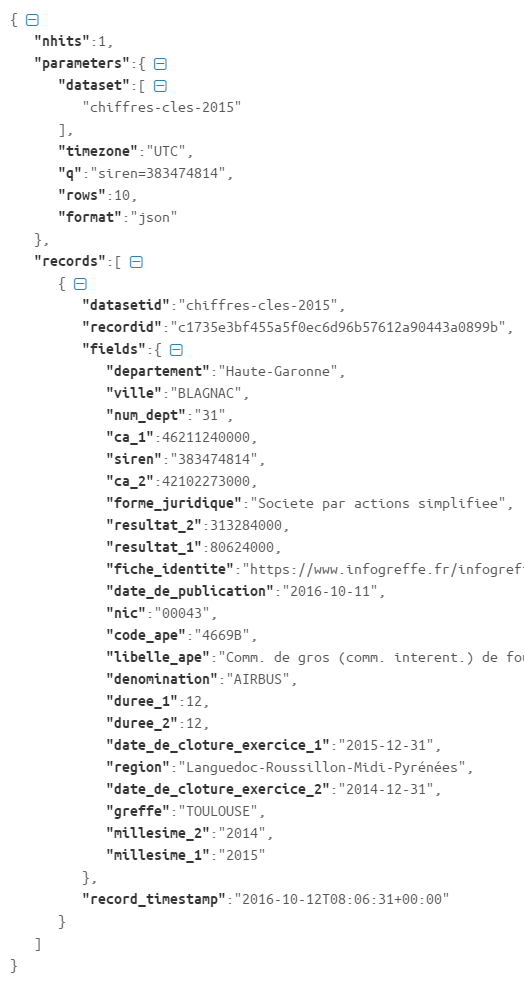
\includegraphics[width=\textwidth, height=400px, draft=false]{annexes/json1.PNG}
\caption{Chiffres clés 2015 de l'entreprise Airbus}
\label{fig3}
\end{figure}

\begin{figure}[ht]
\centering
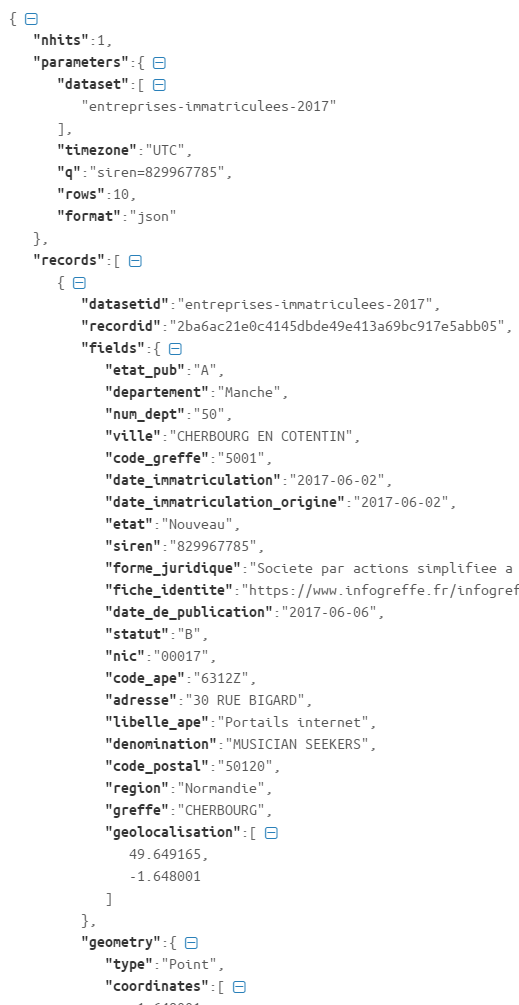
\includegraphics[width=\textwidth, height=500px, draft=false]{annexes/json2.PNG}
\caption{Informations d'immatriculation de l'entreprise Musician Seekers}
\label{fig4}
\end{figure}

\end{appendices}

}
\end{document}
